\documentclass[11pt]{article}
\usepackage[left=2.5cm,right=2.5cm,top=3cm,bottom=3cm,a4paper]{geometry}
\usepackage{enumerate,listings,color,graphicx,subfig}
\usepackage[T1]{fontenc}
\graphicspath{{1-pdf/}}

\definecolor{btgreen}{rgb}{0.1,0.75,0.1}
\definecolor{dkblue}{rgb}{0.25,0.1,0.95}
\definecolor{gray}{rgb}{0.5,0.5,0.5}
\definecolor{mauve}{rgb}{0.58,0,0.82}
\definecolor{brown}{rgb}{0.75,0.2,0.1}
\definecolor{nut}{rgb}{0.8,0.5,0.15}

\lstset{
  frame=tb,
  language=C,
  aboveskip=3mm,
  belowskip=3mm,
  showstringspaces=false,
  columns=flexible,
  basicstyle={\small\ttfamily},
  numbers=none,
  numberstyle=\tiny\color{gray},
  keywordstyle=\color{btgreen},
  commentstyle=\color{dkblue},
  stringstyle=\color{brown},
  breaklines=true,
  breakatwhitespace=true,
  tabsize=3
}
\begin{document}
\section{HEP tutorial: Solution}
The trigger for this tutorial selects events which contain one or more muons as discussed in the documentation and explanation.

\paragraph{1.1}
Find out how often there is more than one isolated, reconstructed muon in data(histogram of the muon multiplicity)! Where could these additional muons come from?\\\\
You should load the data from data.root:
\begin{lstlisting}[emph={if,while,continue,new},emphstyle=\color{nut}]
//exercise1.C
void exercise1(){

  TFile fileIn("files/data.root");
  TTree* theTree = nullptr;
  TTreeReader theReader("events",&fileIn);
  TTreeReaderValue<Int_t> NMuon(theReader, "NMuon");
  TTreeReaderValue<Float_t> EventWeight(theReader, "EventWeight");

  TH1F * h_muon_multi = new TH1F("h_muon_multi","h_muon_multi",10,0,10);

  int nevents = 0;
  while(theReader.Next()){

    float w = *EventWeight;

    int nmuon = *NMuon;
    h_muon_multi->Fill(nmuon,w);

    nevents++;
  }

  int num_muon_0 = h_muon_multi->GetBinContent(1);
  int num_muon_1 = h_muon_multi->GetBinContent(2);
  int num_muon_2 = h_muon_multi->GetBinContent(3);
  int num_muon_3 = h_muon_multi->GetBinContent(4);
  cout << "num. of events with 0 muons = " << num_muon_0 << endl;
  cout << "num. of events with 1 muons = " << num_muon_1 << endl;
  cout << "num. of events with 2 muons = " << num_muon_2 << endl;
  cout << "num. of events with 3 muons = " << num_muon_3 << endl;

  cout << "total number of events = " << nevents << endl;
 
  TFile * f_out = new TFile("out/ex1/hist_data.root","RECERATE");
  h_muon_multi->Wirte();
  f_out->Close();

}
\end{lstlisting}
If you run the upper code, you can get:
\begin{lstlisting}[emph={if,while,continue,new},emphstyle=\color{nut}]
root [0] 
Processing exercise1.C...
num. of events with 0 muons = 227265
num. of events with 1 muons = 223411
num. of events with 2 muons = 18707
num. of events with 3 muons = 1

total number of events = 469384
\end{lstlisting}
and you want to get histogram of the muon multiplicity of data:
\begin{lstlisting}[emph={if,while,continue,new},emphstyle=\color{nut}]
//ex1_multiplot.C
void ex1_multiplot(){

  TFile * f_data = new TFile("out/ex1/hist_data.root");

  TH1F * h_muon_multi_data = (TH1F*) f_data->Get("h_muon_multi");
  h_muon_multi_data->SetMarkerColor(1);

  TCanvas *ex1 = new TCanvas("ex1","ex1",800,600);
  h_muon_multi_data->SetMarkerStyle(20);
  h_muon_multi_data->SetMarkerSize(0.8);
  h_muon_multi_data->Draw("hist");
  h_muon_multi_data->SetStats(0);
  TLegend *leg = new TLegend(.7,.8,.9,.9,"");
  leg->AddEntry(h_muon_multi_data,"data","F");
  leg->Draw();
  ex1->SetLogy();
  h_muon_multi_data->GetYaxis()->SetTitle("Events");
  h_muon_multi_data->GetXaxis()->SetTitle("Number of Muons");
  ex1->Print("out/ex1/muon_multi.pdf");

}

\end{lstlisting}
and the you can get this histogram:
\begin{figure}[h]
\centering
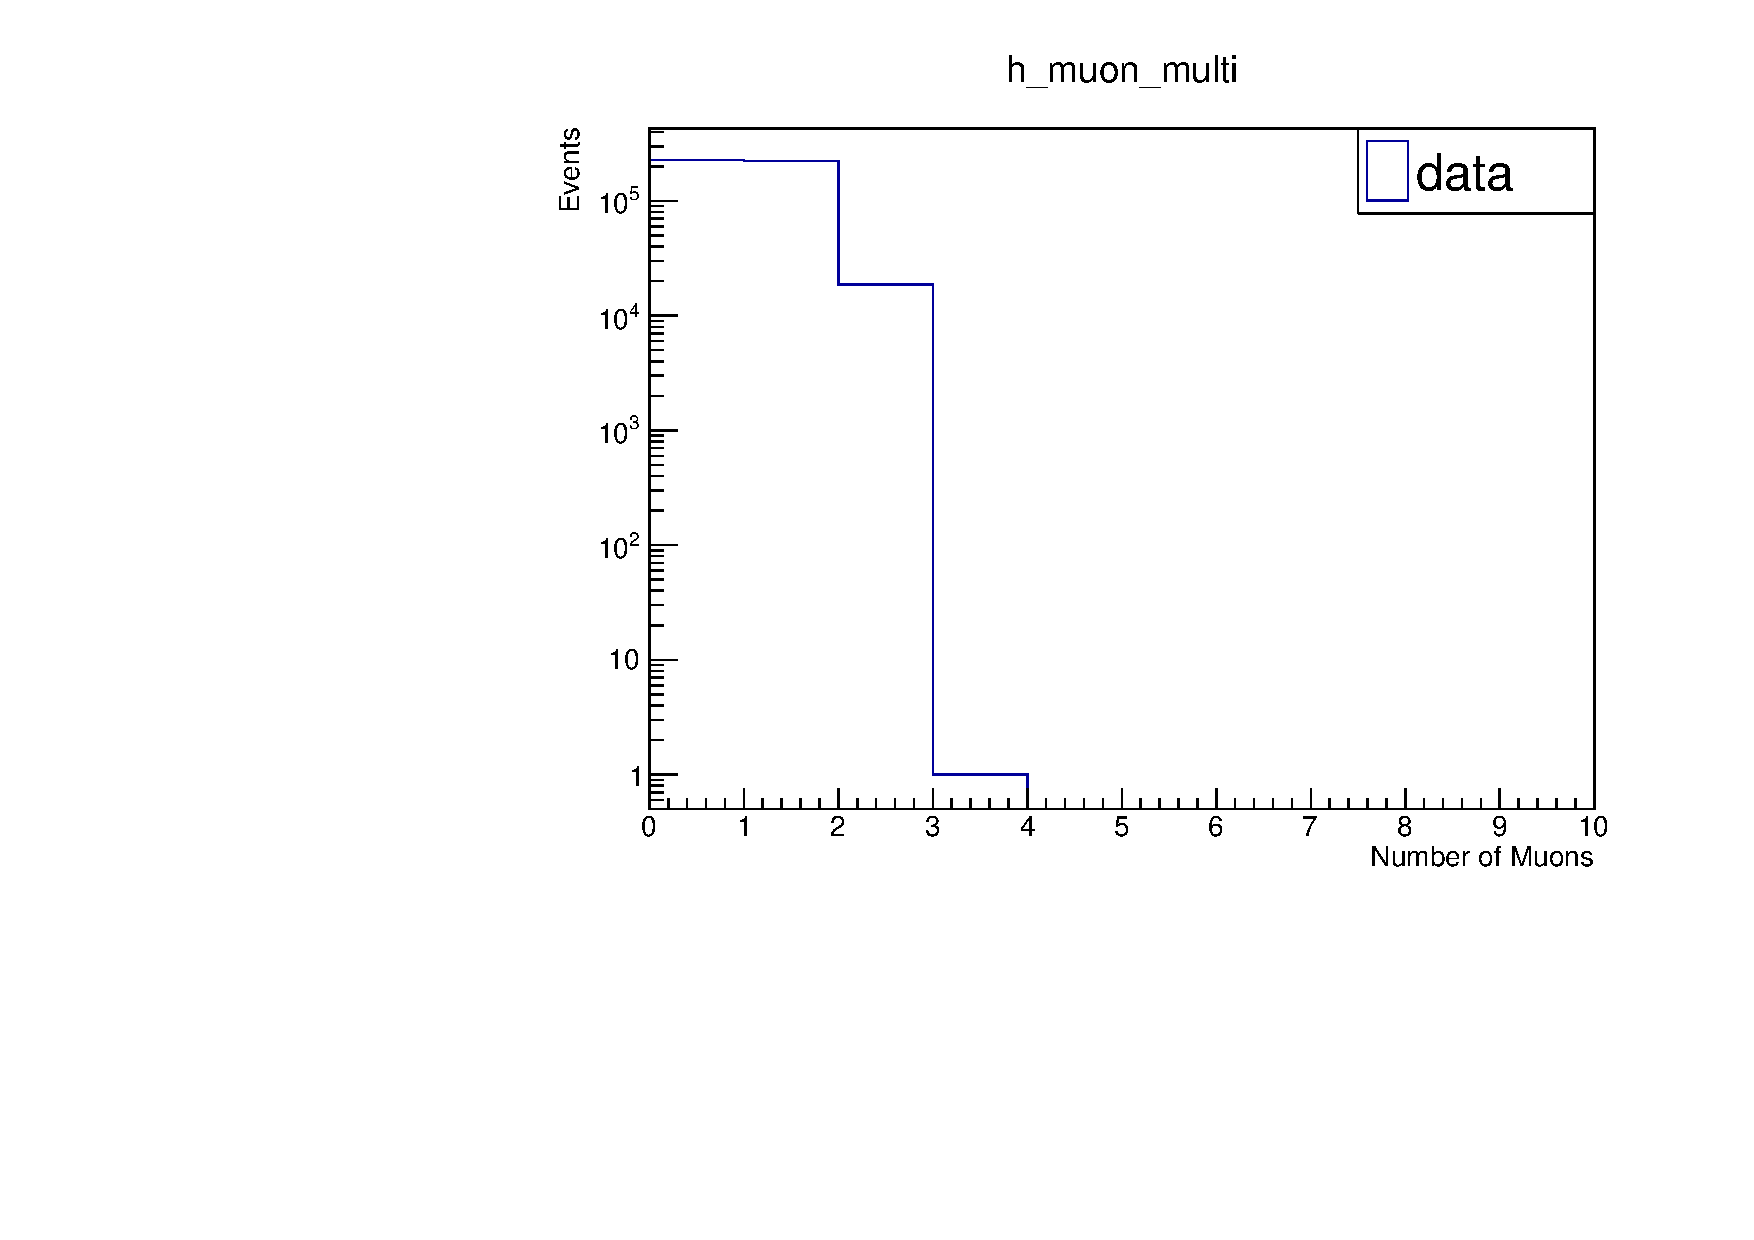
\includegraphics[width=15cm]{muon_multi_data.pdf}
\end{figure}

\newpage
\paragraph{1.2}
Calculate the invariant mass of two muons of opposite charge (manually and/or using the ROOT functionality of adding two fourvectors)! Only use isolated muons.\\\\
You should load some more information:
\begin{lstlisting}[emph={if,while,continue,new},emphstyle=\color{nut}]
//exercise1.C
void exercise1(){

  TFile fileIn("files/data.root");
  TTree* theTree = nullptr;
  TTreeReader theReader("events",&fileIn);
  TTreeReaderValue<Int_t> NMuon(theReader, "NMuon");
  TTreeReaderValue<Float_t> EventWeight(theReader, "EventWeight");
  TTreeReaderArray<Float_t> Muon_Px(theReader, "Muon_Px");
  TTreeReaderArray<Float_t> Muon_Py(theReader, "Muon_Py");
  TTreeReaderArray<Float_t> Muon_Pz(theReader, "Muon_Pz");
  TTreeReaderArray<Float_t> Muon_E(theReader, "Muon_E");
  TTreeReaderArray<Float_t> Muon_Iso(theReader, "Muon_Iso");
  TTreeReaderArray<Int_t> Muon_Charge(theReader, "Muon_Charge");

  TH1F * h_muon_multi = new TH1F("h_muon_multi","h_muon_multi",10,0,10);
  TH1F * h_invmass = new TH1F("h_invmass","h_invmass",120,60,120);

  int nevents = 0;
  while(theReader.Next()){

    float w = *EventWeight;

    int nmuon = *NMuon;
    h_muon_multi->Fill(nmuon,w);

    if(nmuon <= 1) continue;

    float muon1_px = Muon_Px[0];
    float muon1_py = Muon_Py[0];
    float muon1_pz = Muon_Pz[0];
    float muon1_e = Muon_E[0];
    int muon1_charge = Muon_Charge[0]; 

    float muon2_px = Muon_Px[1];
    float muon2_py = Muon_Py[1];
    float muon2_pz = Muon_Pz[1];
    float muon2_e = Muon_E[1];
    int muon2_charge = Muon_Charge[1];

    int muon1_iso = Muon_Iso[0];
    int muon2_iso = Muon_Iso[1];

    if(muon1_iso > 0.1) continue;
    if(muon2_iso > 0.1) continue;
    if(muon1_charge * muon2_charge == 1) continue;

    TLorentzVector P1;
    TLorentzVector P2;
    P1.SetPxPyPzE(muon1_px, muon1_py, muon1_pz, muon1_e);
    P2.SetPxPyPzE(muon2_px, muon2_py, muon2_pz, muon2_e);

    float muon1_pt = P1.Pt();
    float muon2_pt = P2.Pt();

    float dimuon_invmass = (P1 + P2).M();

    h_invmass->Fill(dimuon_invmass,w);

    nevents++;

  }

  TFile * f_out = new TFile("out/ex1/hist_data.root","RECREATE");
  h_muon_multi->Write();
  h_invmass->Write();
  f_out->Close();

}

\end{lstlisting}
histogram is saved.
\newpage
\paragraph{1.3}
Display the invariant mass distribution of two muons in a histogram (hint: try different axis ranges)!\\\\
Do the same work as the muon multiplicity:
\begin{lstlisting}[emph={if,while,continue,new},emphstyle=\color{nut}]
//ex1_invmassplot.C
void ex1_invmassplot(){

  TFile * f_data = new TFile("out/ex1/hist_data.root");

  TH1F * h_invmass_data = (TH1F*) f_data->Get("h_invmass");
  h_invmass_data->SetMarkerColor(1);

  TCanvas *ex1 = new TCanvas("ex1","ex1",800,600);
  h_invmass_data->SetMarkerStyle(20);
  h_invmass_data->SetMarkerSize(0.8);
  h_invmass_data->Draw("hist");
  h_invmass_data->SetStats(0);
  TLegend *leg = new TLegend(.7,.8,.9,.9,"");
  leg->AddEntry(h_invmass_data,"data","F");
  leg->Draw();
  ex1->SetLogy();
  h_invmass_data->GetYaxis()->SetTitle("Events");
  h_invmass_data->GetXaxis()->SetTitle("Muon(GeV)");
  ex1->Print("out/ex1/invmass.pdf");

}
\end{lstlisting}
then you will get
\begin{figure}[h]
\centering
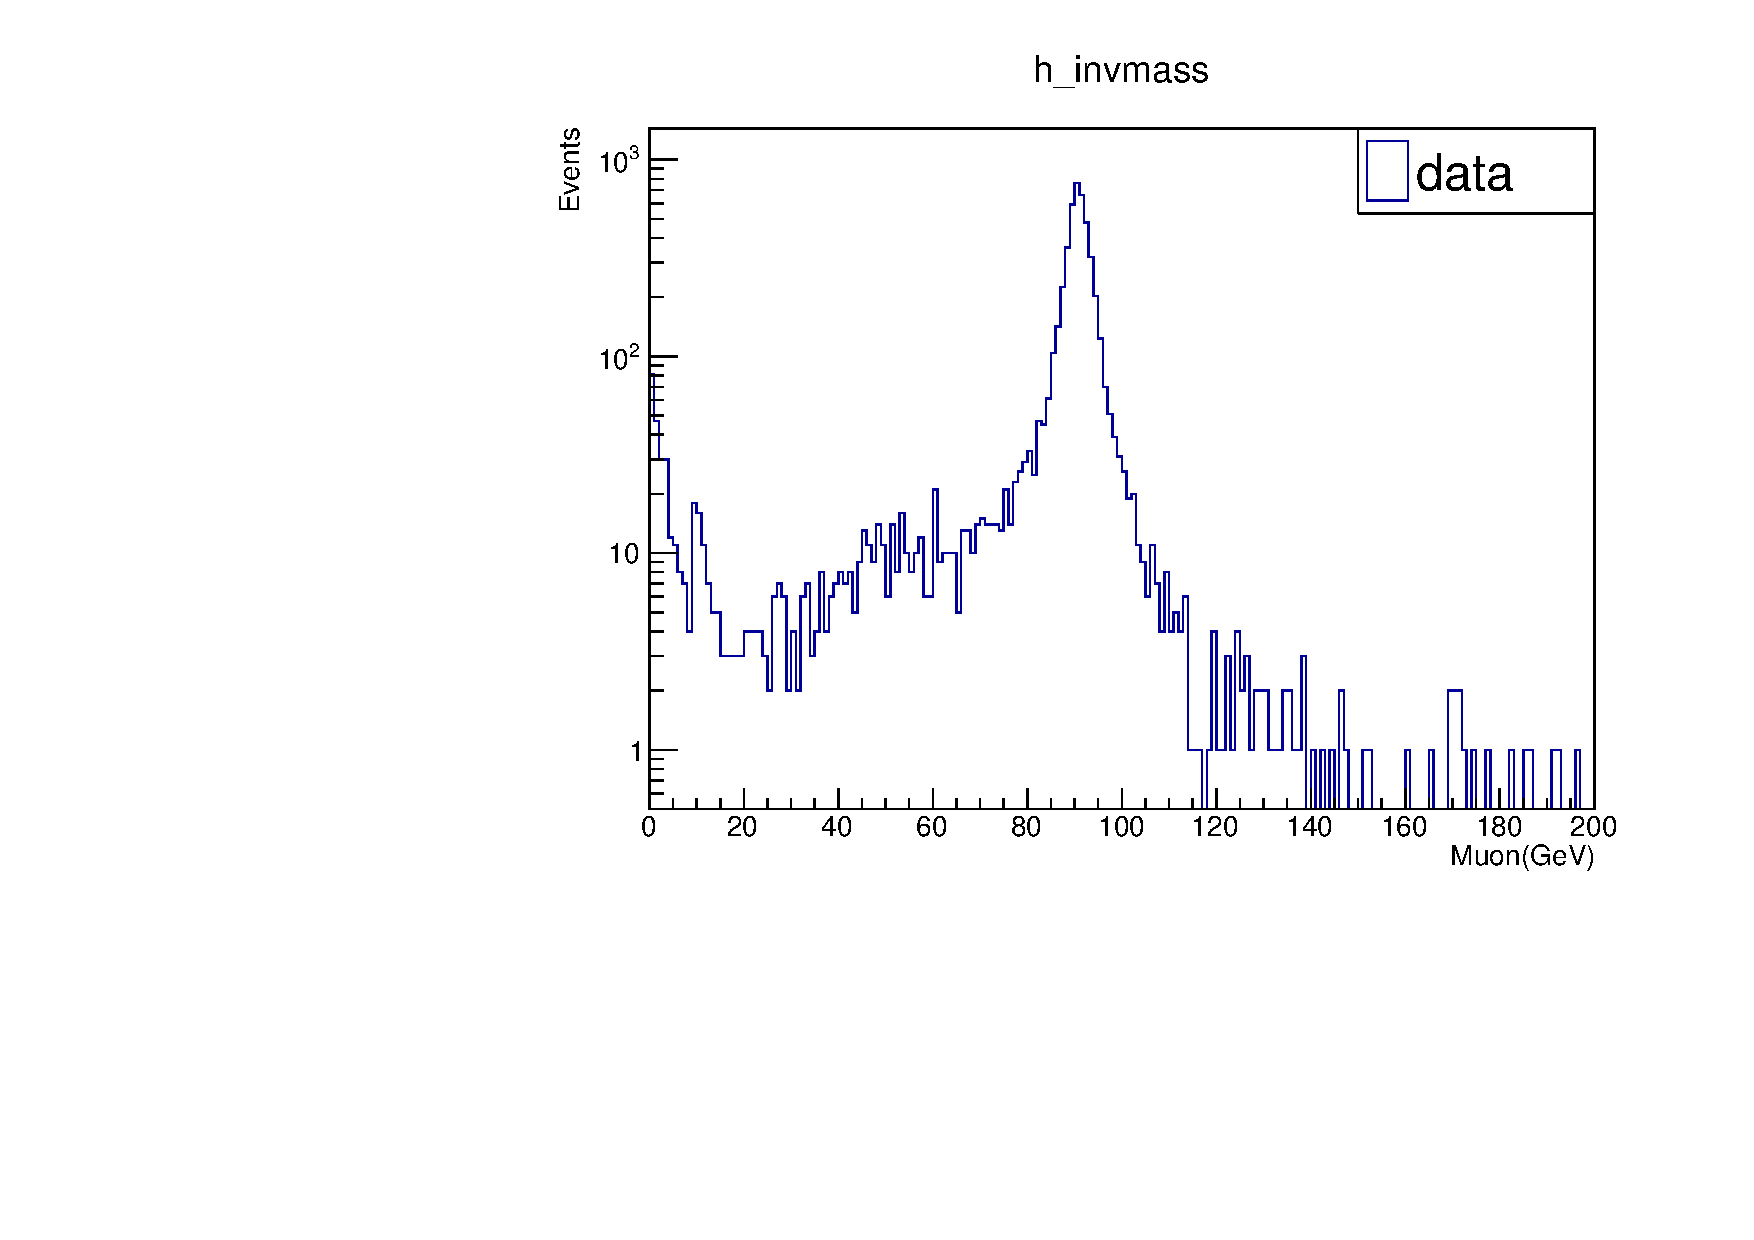
\includegraphics[width=15cm]{invmass_data.pdf}
\end{figure}

\newpage

\paragraph{1.4}
Compare your results to MC simulation (display simulation and data in the same histogram.) Make sure you select triggered events only for the simulated samples!
\\\\
Add information of triggered events
\begin{lstlisting}[emph={if,while,continue,new},emphstyle=\color{nut}]
//exercise1.C
void exercise1(){

  TFile fileIn("files/data.root");
  TTree* theTree = nullptr;
  TTreeReader theReader("events",&fileIn);
  TTreeReaderValue<Int_t> NMuon(theReader, "NMuon");
  TTreeReaderValue<Float_t> EventWeight(theReader, "EventWeight");
  TTreeReaderArray<Float_t> Muon_Px(theReader, "Muon_Px");
  TTreeReaderArray<Float_t> Muon_Py(theReader, "Muon_Py");
  TTreeReaderArray<Float_t> Muon_Pz(theReader, "Muon_Pz");
  TTreeReaderArray<Float_t> Muon_E(theReader, "Muon_E");
  TTreeReaderArray<Float_t> Muon_Iso(theReader, "Muon_Iso");
  TTreeReaderArray<Int_t> Muon_Charge(theReader, "Muon_Charge");

  TH1F * h_muon_multi = new TH1F("h_muon_multi","h_muon_multi",10,0,10);
  TH1F * h_invmass = new TH1F("h_invmass","h_invmass",120,60,120);

  int nevents = 0;
  while(theReader.Next()){
  
    float w = *EventWeight;
  
    int nmuon = *NMuon;
    h_muon_multi->Fill(nmuon,w);

    if(nmuon <= 1) continue;

    float muon1_px = Muon_Px[0];
    float muon1_py = Muon_Py[0];
    float muon1_pz = Muon_Pz[0];
    float muon1_e = Muon_E[0];
    int muon1_charge = Muon_Charge[0];

    float muon2_px = Muon_Px[1];
    float muon2_py = Muon_Py[1];
    float muon2_pz = Muon_Pz[1];
    float muon1_e = Muon_E[0];
    int muon1_charge = Muon_Charge[0];

    float muon2_px = Muon_Px[1];
    float muon2_py = Muon_Py[1];
    float muon2_pz = Muon_Pz[1];
    float muon2_e = Muon_E[1];
    int muon2_charge = Muon_Charge[1];

    int muon1_iso = Muon_Iso[0];
    int muon2_iso = Muon_Iso[1];
    bool muon_tri = *Muon_trigger;

    if(muon1_iso > 0.1) continue;
    if(muon2_iso > 0.1) continue;
    if(muon1_charge * muon2_charge == 1) continue;
    if(muon_tri == false) continue;

    TLorentzVector P1;
    TLorentzVector P2;
    P1.SetPxPyPzE(muon1_px, muon1_py, muon1_pz, muon1_e);
    P2.SetPxPyPzE(muon2_px, muon2_py, muon2_pz, muon2_e);

    float muon1_pt = P1.Pt();
    float muon2_pt = P2.Pt();

    float dimuon_invmass = (P1 + P2).M();

    h_invmass->Fill(dimuon_invmass,w);

    nevents++;

  }

  TFile * f_out = new TFile("out/ex1/hist_data.root","RECREATE");
  h_muon_multi->Write();
  h_invmass->Write();
  f_out->Close();

}

\end{lstlisting}
Now you want to do the same work not only for data, but for ttbar, Drell-Yan and so on. You can change this:
\begin{lstlisting}[emph={if,while,continue,new},emphstyle=\color{nut}]
//exercise1.C
void exercise1(){

  TFile fileIn("files/data.root");

  .
  .
  .

  TFile * f_out = new TFile("out/ex1/hist_data","RECREATE"); 
  h_muon_multi->Write();
  h_invmass->Write();
  f_out->Close();

}

\end{lstlisting}
to this:
\begin{lstlisting}[emph={if,while,continue,new},emphstyle=\color{nut}]

void exericise1(string inputFile){

  TFile fileIn(Form("files/%s",inputFile.c_str()));

  .
  .
  .

  TFile * f_out = new TFile(Form("out/hist_%s",inputFile.c_str()),"RECREATE"); 
  h_muon_multi->Write();
  h_invmass->Write();
  f_out->Close();
}

\end{lstlisting}
and follow this code and change the permission.
\begin{lstlisting}[emph={if,while,continue,new},emphstyle=\color{nut}]
//job_ex1.sh
#! /bin/bash

root -l -b -q exercise1.C'("ww.root")'
root -l -b -q exercise1.C'("zz.root")'
root -l -b -q exercise1.C'("wz.root")'
root -l -b -q exercise1.C'("qcd.root")'
root -l -b -q exercise1.C'("ttbar.root")'
root -l -b -q exercise1.C'("wjets.root")'
root -l -b -q exercise1.C'("single_top.root")'
root -l -b -q exercise1.C'("dy.root")'
root -l -b -q exercise1.C'("data.root")'


\end{lstlisting}
and then the root files will be produced
\begin{lstlisting}[emph={if,while,continue,new},emphstyle=\color{nut}]

Processing exercise1.C("ww.root")...

Processing exercise1.C("zz.root")...

Processing exercise1.C("wz.root")...

Processing exercise1.C("qcd.root")...

Processing exercise1.C("ttbar.root")...

Processing exercise1.C("wjets.root")...

Processing exercise1.C("single_top.root")...

Processing exercise1.C("dy.root")...

Processing exercise1.C("data.root")...

\end{lstlisting}
You have to compare your results to MC simulation. 
\begin{lstlisting}[emph={if,while,continue,new},emphstyle=\color{nut}]
//stack_ex1.C
void stack_ex1(){

  TFile * f_data = new TFile("out/ex1/hist_data.root");
  TFile * f_dy = new TFile("out/ex1/hist_dy.root");
  TFile * f_ttbar = new TFile("out/ex1/hist_ttbar.root");
  TFile * f_qcd = new TFile("out/ex1/hist_qcd.root");
  TFile * f_wjets = new TFile("out/ex1/hist_wjets.root");
  TFile * f_single_top = new TFile("out/ex1/hist_single_top.root");
  TFile * f_ww = new TFile("out/ex1/hist_ww.root");
  TFile * f_wz = new TFile("out/ex1/hist_wz.root");
  TFile * f_zz = new TFile("out/ex1/hist_zz.root");

  THStack *sh = new THStack("sh","multi");
  TH1F * h_muon_multi_ttbar = (TH1F*) f_ttbar->Get("h_muon_multi");
  TH1F * h_muon_multi_dy = (TH1F*) f_dy->Get("h_muon_multi");
  TH1F * h_muon_multi_qcd = (TH1F*) f_qcd->Get("h_muon_multi");
  TH1F * h_muon_multi_wjets = (TH1F*) f_wjets->Get("h_muon_multi");
  TH1F * h_muon_multi_ww = (TH1F*) f_ww->Get("h_muon_multi");
  TH1F * h_muon_multi_wz = (TH1F*) f_wz->Get("h_muon_multi");
  TH1F * h_muon_multi_zz = (TH1F*) f_zz->Get("h_muon_multi");
  TH1F * h_muon_multi_single_top = (TH1F*) f_single_top->Get("h_muon_multi");
  TH1F * h_muon_multi_data = (TH1F*) f_data->Get("h_muon_multi");

  h_muon_multi_ttbar->SetFillColor(kRed);
  h_muon_multi_wjets->SetFillColor(kOrange);
  h_muon_multi_dy->SetFillColor(kBlue);
  h_muon_multi_ww->SetFillColor(kGreen);
  h_muon_multi_wz->SetFillColor(kCyan);
  h_muon_multi_zz->SetFillColor(kYellow);
  h_muon_multi_qcd->SetFillColor(kMagenta);
  h_muon_multi_single_top->SetFillColor(kGray);
  h_muon_multi_data->SetMarkerColor(1);

  sh->Add(h_muon_multi_ttbar);
  sh->Add(h_muon_multi_wjets);
  sh->Add(h_muon_multi_dy);
  sh->Add(h_muon_multi_ww);
  sh->Add(h_muon_multi_wz);
  sh->Add(h_muon_multi_zz);
  sh->Add(h_muon_multi_qcd);
  sh->Add(h_muon_multi_single_top);

  TCanvas *fstack = new TCanvas("fstack","multi",700,600);
  h_muon_multi_data->SetMarkerStyle(20);
  h_muon_multi_data->SetLineColor(1);
  h_muon_multi_data->SetMarkerSize(0.8);
  fstack->DrawFrame(0,0.5,7,1000000)->SetTitle("muon multiplicity");
  sh->GetYaxis()->SetTitle("Events");
  sh->GetXaxis()->SetTitle("Number of Muon");
  sh->Draw("histsame");
  h_muon_multi_data->Draw("psame");
  TLegend *leg = new TLegend(.75,.55,.9,.9,"");
  leg->AddEntry(h_muon_multi_ttbar,"ttbar","F");
  leg->AddEntry(h_muon_multi_wjets,"wjets","F");
  leg->AddEntry(h_muon_multi_dy,"Drell-Yan","F");
  leg->AddEntry(h_muon_multi_ww,"ww","F");
  leg->AddEntry(h_muon_multi_wz,"wz","F");
  leg->AddEntry(h_muon_multi_zz,"zz","F");
  leg->AddEntry(h_muon_multi_qcd,"qcd","F");
  leg->AddEntry(h_muon_multi_single_top,"single_top","F");
  leg->AddEntry(h_muon_multi_data,"data","p");
  leg->Draw();
  fstack->SetLogy();
  fstack->Print("out/ex1/STACK_multi.pdf");

  THStack *hs = new THStack("hs","invariant mass");
  TH1F * h_invmass_ttbar = (TH1F*) f_ttbar->Get("h_invmass");
  TH1F * h_invmass_dy = (TH1F*) f_dy->Get("h_invmass");
  TH1F * h_invmass_qcd = (TH1F*) f_qcd->Get("h_invmass");
  TH1F * h_invmass_wjets = (TH1F*) f_wjets->Get("h_invmass");
  TH1F * h_invmass_ww = (TH1F*) f_ww->Get("h_invmass");
  TH1F * h_invmass_wz = (TH1F*) f_wz->Get("h_invmass");
  TH1F * h_invmass_zz = (TH1F*) f_zz->Get("h_invmass");
  TH1F * h_invmass_single_top = (TH1F*) f_single_top->Get("h_invmass");
  TH1F * h_invmass_data = (TH1F*) f_data->Get("h_invmass");

  h_invmass_ttbar->SetFillColor(kRed);
  h_invmass_wjets->SetFillColor(kOrange);
  h_invmass_dy->SetFillColor(kBlue);
  h_invmass_ww->SetFillColor(kGreen);
  h_invmass_wz->SetFillColor(kCyan);
  h_invmass_zz->SetFillColor(kYellow);
  h_invmass_qcd->SetFillColor(kMagenta);
  h_invmass_single_top->SetFillColor(kGray);
  h_invmass_data->SetMarkerColor(1);

  hs->Add(h_invmass_ttbar);
  hs->Add(h_invmass_wjets);
  hs->Add(h_invmass_dy);
  hs->Add(h_invmass_ww);
  hs->Add(h_invmass_wz);
  hs->Add(h_invmass_zz);
  hs->Add(h_invmass_qcd);
  hs->Add(h_invmass_single_top);

  TCanvas *sstack = new TCanvas("sstack","invmass",700,600);
  h_invmass_data->SetMarkerStyle(20);
  h_invmass_data->SetMarkerSize(0.8);
  h_invmass_data->SetLineColor(1);
  hs->Draw("hist");
  h_invmass_data->Draw("epsame");
  TLegend *leg2 = new TLegend(.75,.55,.9,.9,"");
  leg2->AddEntry(h_invmass_ttbar,"ttbar","F");
  leg2->AddEntry(h_invmass_wjets,"wjets","F");
  leg2->AddEntry(h_invmass_dy,"Drell-Yan","F");
  leg2->AddEntry(h_invmass_ww,"ww","F");
  leg2->AddEntry(h_invmass_wz,"wz","F");
  leg2->AddEntry(h_invmass_zz,"zz","F");
  leg2->AddEntry(h_invmass_qcd,"qcd","F");
  leg2->AddEntry(h_invmass_single_top,"single_top","F");
  leg2->AddEntry(h_invmass_data,"data","p");
  leg2->Draw();
  sstack->SetLogy();
  hs->GetYaxis()->SetTitle("Events");
  hs->GetXaxis()->SetTitle("Muon(GeV)");
  sstack->Print("out/ex1/STACK_invmass.pdf");

}

\end{lstlisting}
Now you can get these histograms:
\begin{figure}[h]
\centering
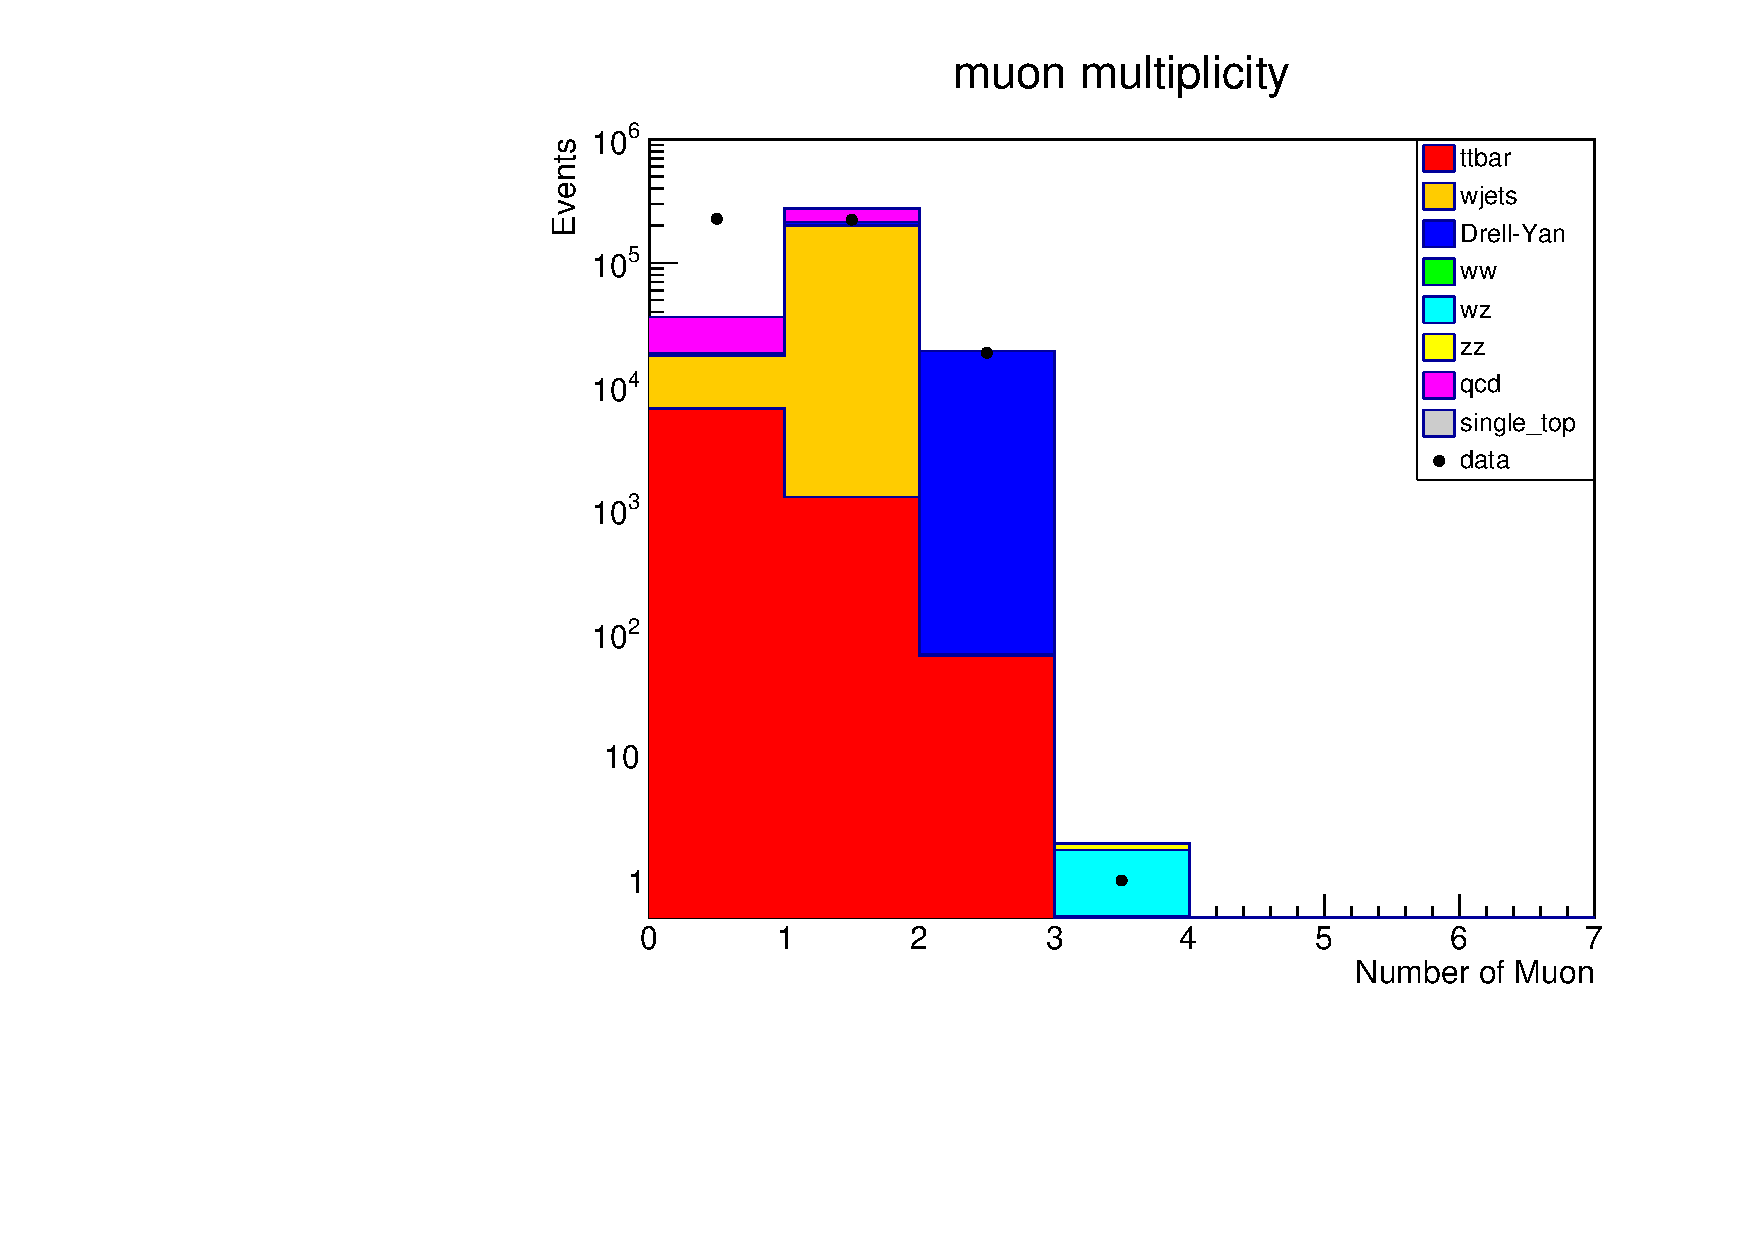
\includegraphics[width=15cm]{STACK_multi.pdf}
\qquad
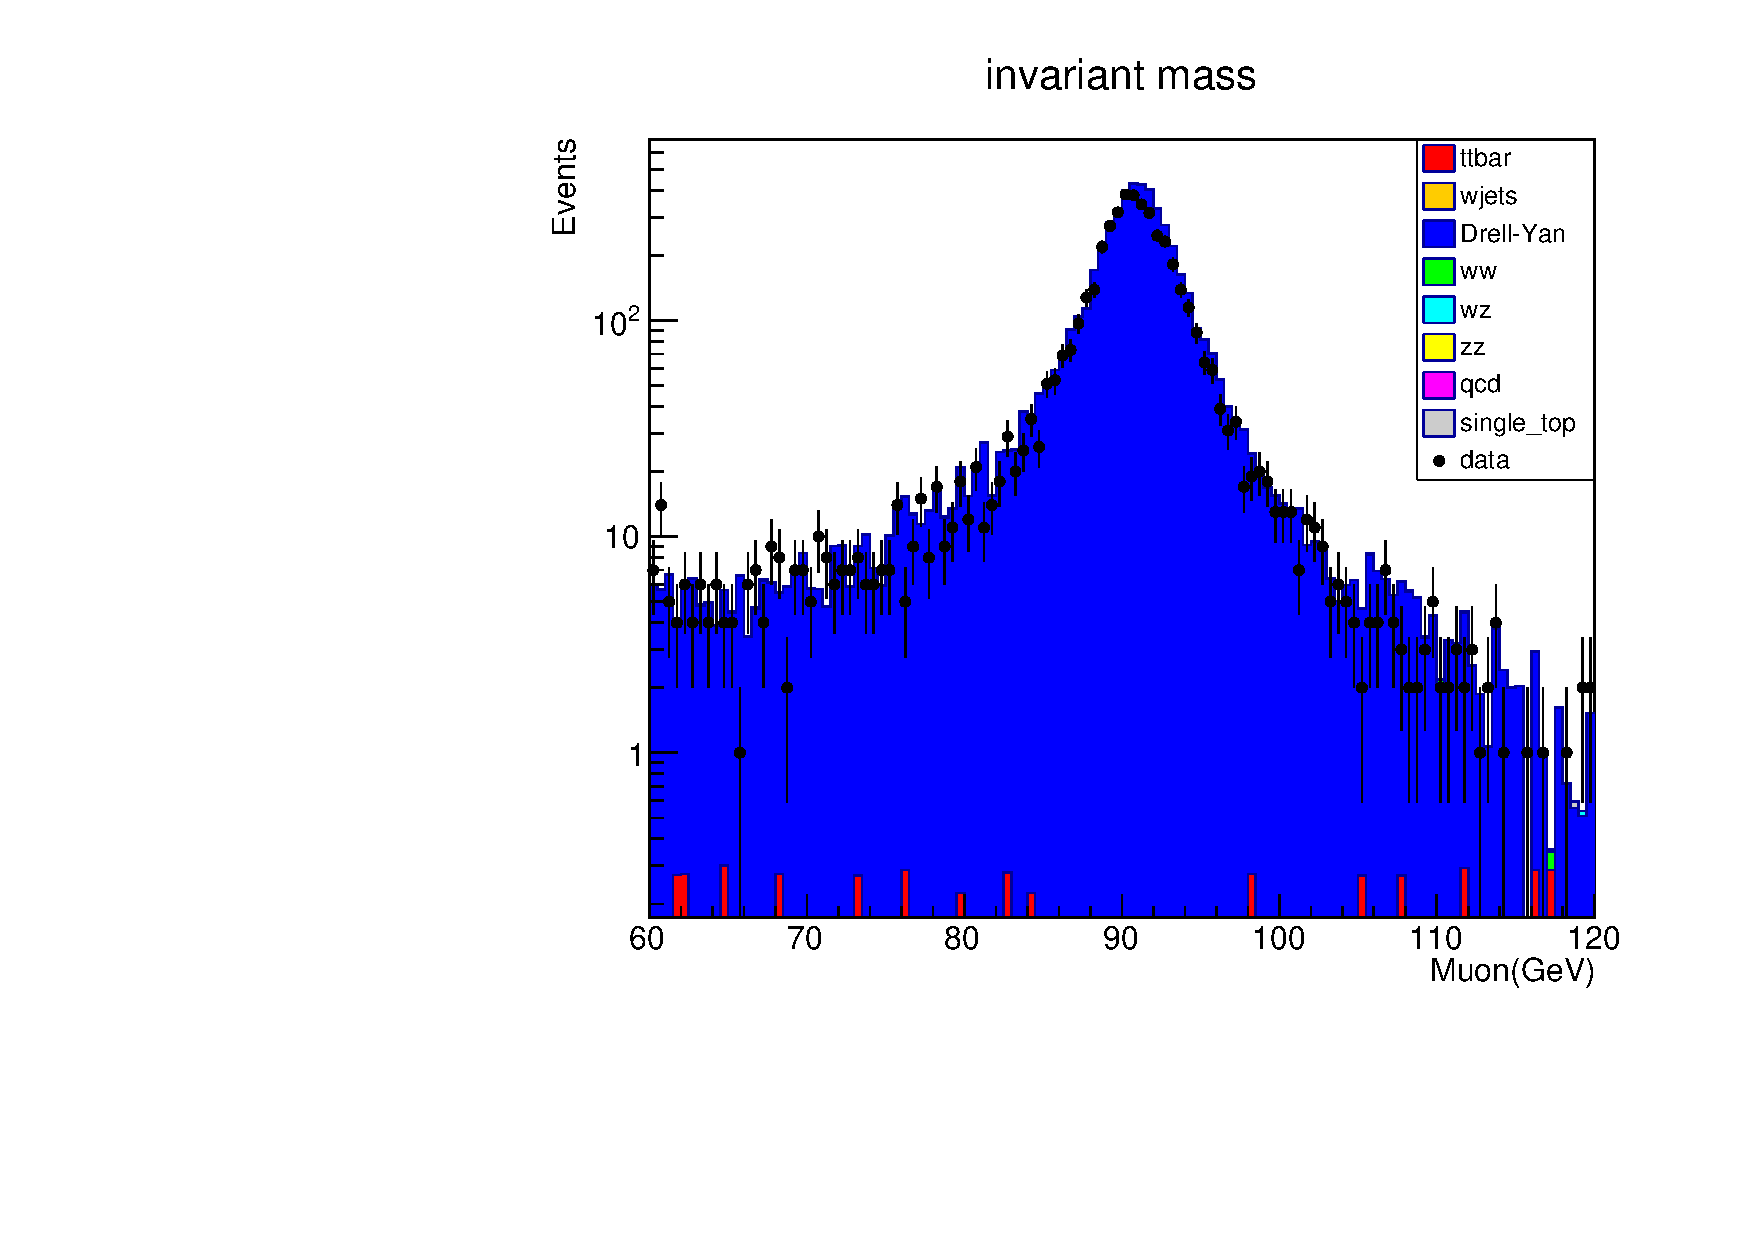
\includegraphics[width=15cm]{STACK_invmass.pdf}
\end{figure}
\end{document}

